\section{Исследование и построение решения задачи}
\subsection{Современные подходы к обработке естественного языка}
За последние несколько лет область обработки текстов значительным образом преобразилась. Тексты хуже поддаются обработке различными нейросетевыми алгоритмами из-за их дискретной структуры. Только в 2013 году с появлением word2vec началось стремительное развитие применения нейросетей в обработке текстов. Основная идея данного подхода заключается в выучивании векторов слов для выполнения дистрибутивной гипотезы: слова, встречающиеся в схожих контекстах, имеют близкие значения.

Долгое время стандартом моделей была одна из векторизаций (word2vec, glove, fasttext) с какой-либо рекуррентной нейросетью (LSTM, GRU) и финальным слоем специфичным для задачи. Со временем начали появляться модели более общего назначения, которые не требовалось обучать с нуля для каждой задачи: Fairseq, ELMo\cite{Peters:2018}, BERT\cite{devlin2018bert}, M-USE.

В настоящий момент большие предобученные модели основанные на архитектуре трансформеров являются доминирующими во всех или почти всех областях обработки текстов. Особенностью данной архитектуры является полный отказ от рекуррентности в пользу механизма внимания.

Механизм внимания пришел из задачи машинного перевода, где главным подходом была архитектура Seq2Seq. Данная архитектура состоит из энкодера, сжимающего предложение в вектор, и декодера, разжимающего данный вектор в текст на другом языке. Одна из главных заявленнных проблем - данный подход плохо работает на длинных предложениях. Это связано с тем, что при сжатии в вектор фиксированного размера теряется очень большой объем информации.

Прорыв произошел с разработкой механизма внимания \cite{bahdanau2014neural}. Данный механизм позволяет сопоставлять вектор предложения в декодере с соответствующими состояними в энкодере. Каждому состоянию энкодера, соответствуещему определенному токену, на каждом шаге декодировке ставится в соответствие вес, после чего состояния энкодера усредняются с данными весами и используются для расширения внутреннего состояния декодера.

\begin{figure}[H]
 \captionsetup{justification=raggedright,singlelinecheck=false,labelfont=bf,labelsep=period,name={Рисунок}}
 \centering{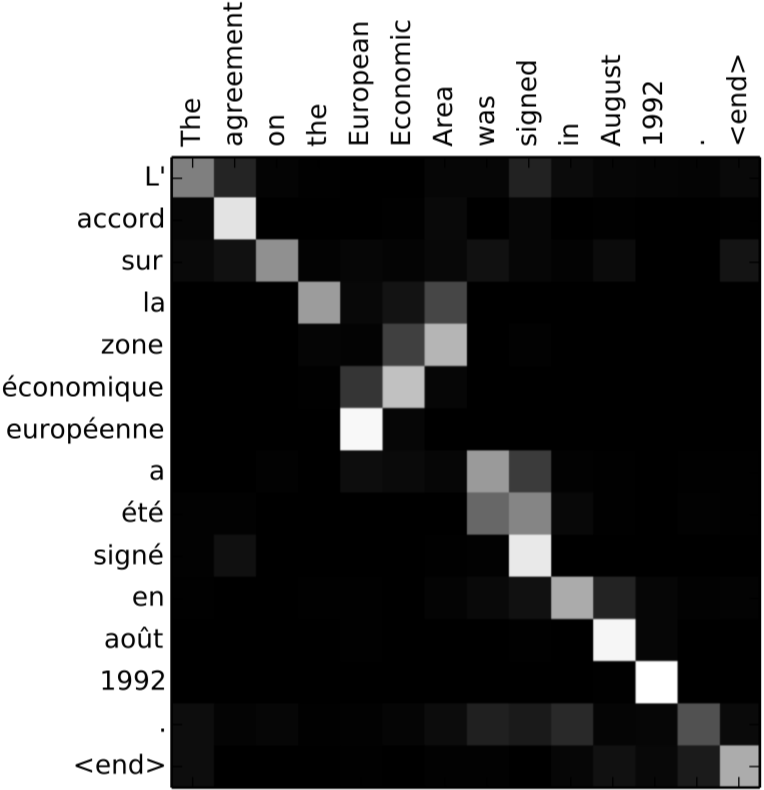
\includegraphics[scale=0.7]{attention.png}}
 \caption{Пример матрицы механизма внимания, полученного при переводе с английского языка на французский.}
\end{figure}

Архитектура трансформера основывается на механизме внимания. При этом в рамках энкодера механизм внимания применяется сам к себе. С последовательным применением нелинейности данный механизм применяется несколько раз на каждом слое нейросети, после чего на выходе получается векторное представление для каждого слова в предложении, насыщенное контекстуальной информацией.

Одной из самых популярных предобученных архитектур является BERT. Данная модель обучалась на Book Corpus задаче маскированного языкового моделирования и предсказания следующего предложения. Задача маскированного языкового  моделирования заключается в предсказании одного и более слов в предложении. Таким образом после обучения модель имеет внутри себя знания о структуре языка, о мире, поэтому ее легко адаптировать для различных вариаций задачи понимания естественного языка (Natural Language Understanding).

Это подтверждается успехом подобных моделей почти во всех современных задачах естественного языка (Natural Language Understanding) и особом соревновании GLUE Benchmark. Данное соревнование содержит в себе ряд задач на понимание языка, которые при небольшом дообучении решаются моделями подобными BERT на уровне человека или выше.

Так как базовые нейросетевые подходы на эмбеддингах GloVe, word2vec и стандартных рекуррентных нейросетях (LSTM, GRU), а также подходы основанные на машинном обучении уже были исследованы, в рамках данной работы исследуется применимость больших предобученных языковых моделей на архитектуре трансформер \cite{vaswani2017attention}.

\subsection{Методы межязыкового переноса знаний}
В научном сообществе наиболее распространены англоязычные корпуса. Этот язык получает наибольшее покрытие задачами, однако остальные языки из-за этого не получают должного внимания.

Методов получить модель для другого языка несколько, направления межязыкового переноса активно развивается в настоящее время. Самым простоым способом является создание параллельного корпуса. Использование профессиональных переводчиков затратно и треюует много времени, поэтому достаточно часто прибегают к автоматизированным средствам перевода.

Второй подход заключается в адаптации мультиязычной модели, т.е. модели предобученной на корпусе из различных языков. Считается, что для представлений одних и тех же слов на разных языках модель имеет схожие векторные представления, которые "замораживаются", т.е. не обучаются дальше. После этого данная модель дообучается на конкретной задаче на тех языках, на которых данная задача доступна, а качество замеряется уже на целевом языке.

\begin{figure}[H]
 \captionsetup{justification=raggedright,singlelinecheck=false,labelfont=bf,labelsep=period,name={Рисунок}}
 \centering{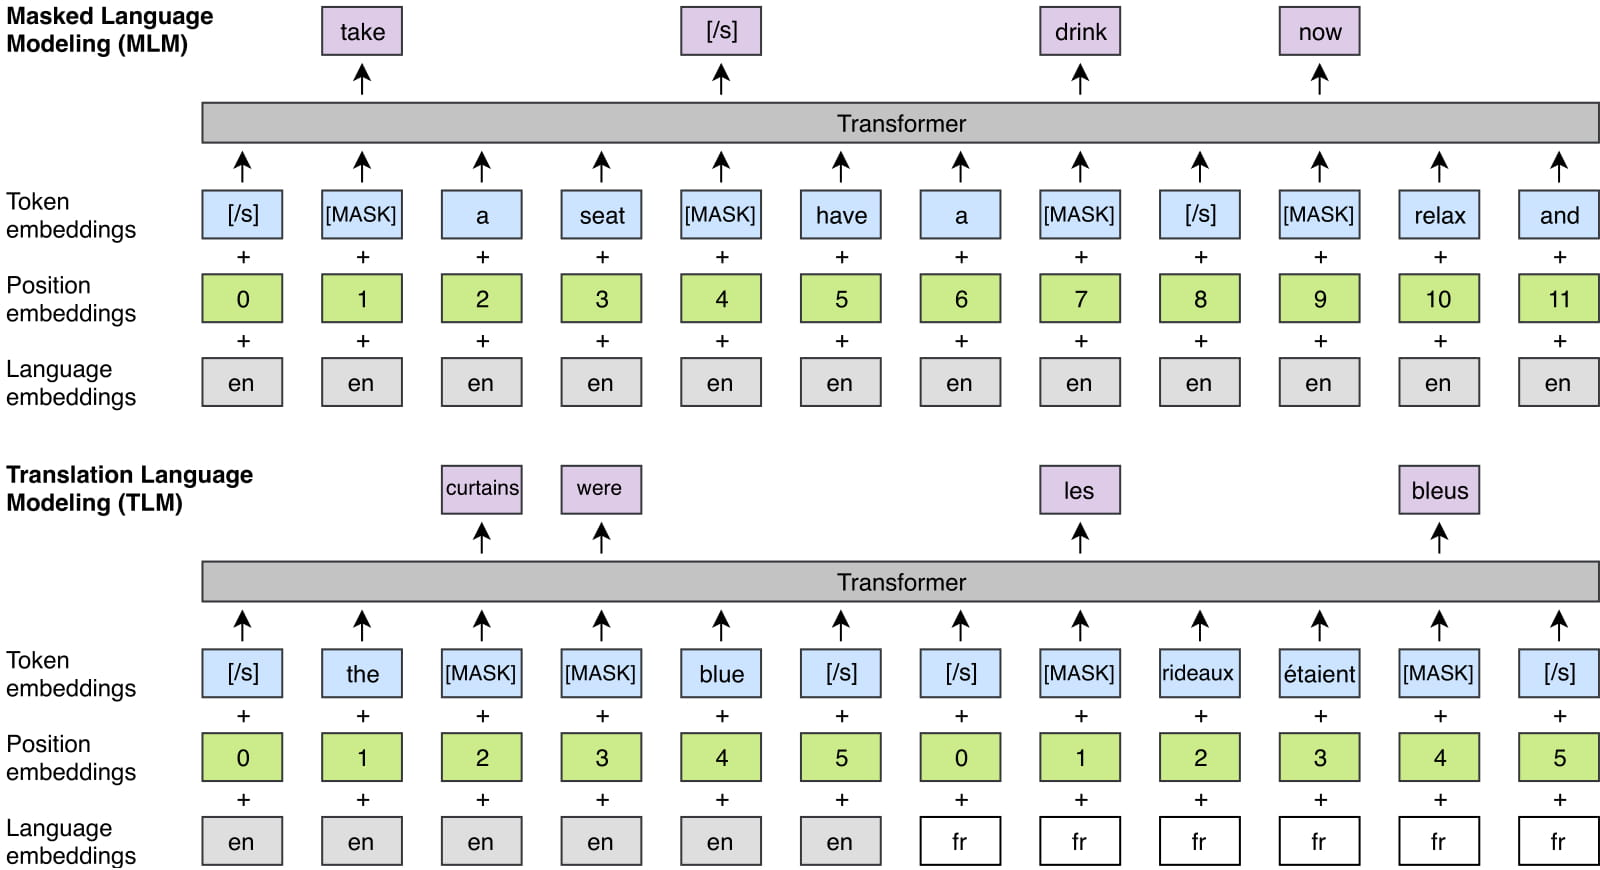
\includegraphics[scale=0.3]{xlm.jpeg}}
 \caption{Процесс предобучения мультиязычной модели XLM.}
\end{figure}

Третий подход состоит в обучении CoVe-векторов для представлений слов. Это вектора, полученные в энкодере архитектуры Seq2Seq на задаче машинного перевода. Данные вектора впоследствие конкатенируются к векторным представлениям слов при решении целевой задачи, чем  обогащают представление слова в  нейросети.

\begin{figure}[H]
 \captionsetup{justification=raggedright,singlelinecheck=false,labelfont=bf,labelsep=period,name={Рисунок}}
 \centering{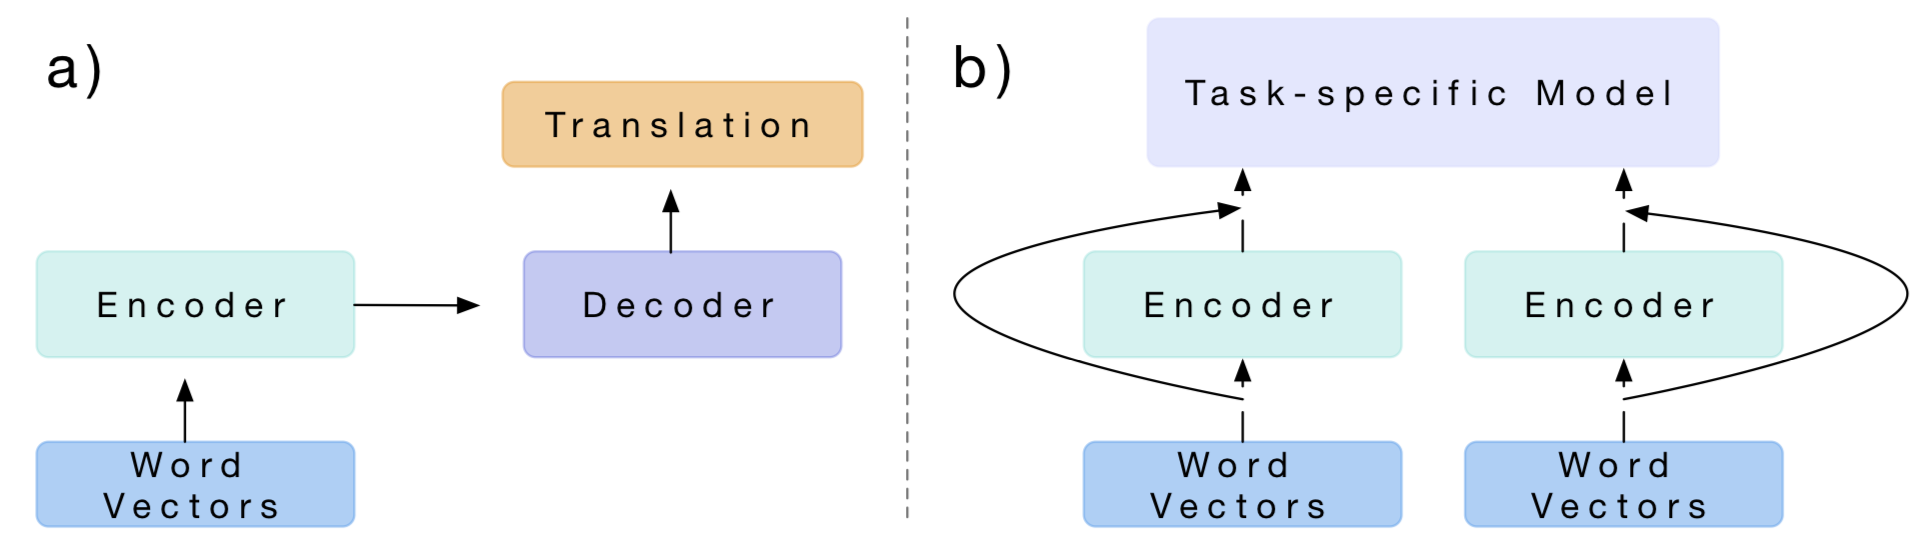
\includegraphics[scale=0.5]{cove.png}}
 \caption{Схема обучения и использования CoVe-векторов. а) - предобучение на задаче машинного перевода, b) - процесс обогащения входных векторов модели с помощью CoVe.}
\end{figure}

\subsection{Выводы}
В результате рассмотрения рассмотрения текущих трендов в области обработки естественного языка было решено использовать для задачи выделения аргументации предобученные языковые модели, так как они на данный момент лидириют почти во всех задачах. Для проблемы переноса знаний на русский язык было попробовать как создание параллельного корпуса с помощью перевода, так и перенос знаний с помощью использования мультязычных языковых моделей. 

Было принято решение не адаптировать подход CoVe из-за вычислительной трудности решения задачи машинного перевода с помощью нейросетей.